\documentclass{article}
\usepackage[english]{babel}
\usepackage[utf8x]{inputenc}
\usepackage[left=2cm,right=2cm,top=2cm,bottom=2cm]{geometry}
\usepackage{amssymb}
\usepackage{amsmath}
\usepackage{graphicx}
\usepackage[colorinlistoftodos]{todonotes}
\usepackage{hyperref}
\usepackage{float}
\usepackage{systeme}
\newcommand\tab[1][1cm]{\hspace*{#1}}
\usepackage{booktabs}
\usepackage{hyperref}
\newcommand{\tabitem}{~~\llap{\textbullet}~~}

\begin{document}
\begin{titlepage}
\newcommand{\HRule}{\rule{\linewidth}{0.1mm}} 
\center


\textsc{\Large Equation de Poisson et traitement d'image}\\[0.5cm]
\textsc{\Large Groupe de travail thématique}\\[0.5cm] 
\textsc{4TQMS801S}\\[0.5cm] 


\HRule \\[0.4cm]
{ \huge \bfseries Fichier Annexe, Résultats}\\[0.1cm] % Title of your Homework/assignment
\HRule \\[1.5cm]


\begin{minipage}{1.0\textwidth}
\Large  Virginie MONTALIBET \hfill Sébastien Eyzat 

\end{minipage}
\begin{minipage}{1.0\textwidth}
\end{minipage}\\[1cm]

{\Large \today}\\[1cm]

\includegraphics[width=15cm,  height=6cm,  keepaspectratio]
{Images/logo.png}
\vfill
\end{titlepage}
\begin{figure}[!htb]
   \begin{minipage}{0.33\textwidth}
     \centering
     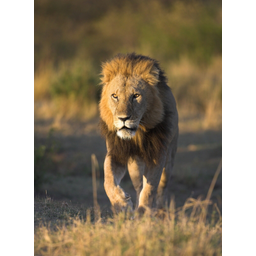
\includegraphics[width = 120pt]{Annexe/lio.png}
     \caption{Image S}
      \end{minipage}\hfill
   \begin{minipage}{0.33\textwidth}
     \centering
     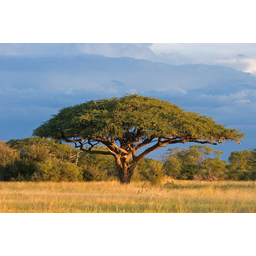
\includegraphics[width = 120pt]{Annexe/arbre.png}
     \caption{Image T}
      \end{minipage}\hfill
      \end{figure}

\begin{figure}[!htb]
   \begin{minipage}{0.33\textwidth}
     \centering
     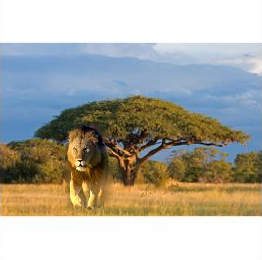
\includegraphics[width = 120pt]{Annexe/LionD.png}
     \caption{Méthode Douglas}
      \end{minipage}\hfill
   \begin{minipage}{0.33\textwidth}
     \centering
     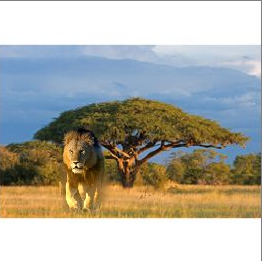
\includegraphics[width = 120pt]{Annexe/LionDF.png}
     \caption{Différences finies}
      \end{minipage}\hfill
   \begin{minipage}{0.33\textwidth}
     \centering
     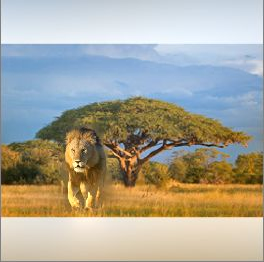
\includegraphics[width= 120pt]{Annexe/LF.png}
     \caption{Fourier}
   \end{minipage}
\end{figure}
%%%%%%%%%%%%%%%%%%%%%REQUIN
\begin{figure}[!htb]
   \begin{minipage}{0.5\textwidth}
     \centering
     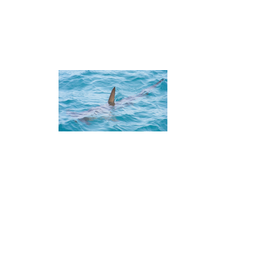
\includegraphics[width = 120pt]{Annexe/requin.png}
     \caption{Image S}
      \end{minipage}\hfill
   \begin{minipage}{0.33\textwidth}
     \centering
     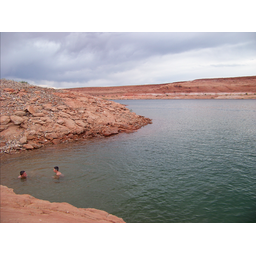
\includegraphics[width = 120pt]{Annexe/ocean.png}
     \caption{Image T}
      \end{minipage}\hfill
      \end{figure}

\begin{figure}[!htb]
   \begin{minipage}{0.33\textwidth}
     \centering
     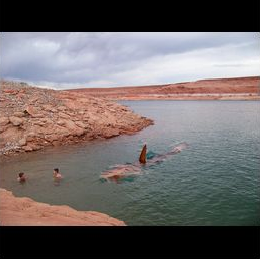
\includegraphics[width = 120pt]{Annexe/RequinD.png}
     \caption{Méthode Douglas}
      \end{minipage}\hfill
   \begin{minipage}{0.33\textwidth}
     \centering
     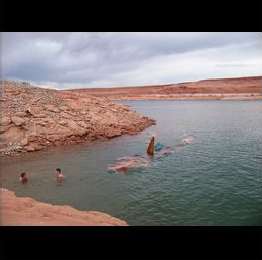
\includegraphics[width = 120pt]{Annexe/requinDF.png}
     \caption{Différences finies}
      \end{minipage}\hfill
   \begin{minipage}{0.33\textwidth}
     \centering
     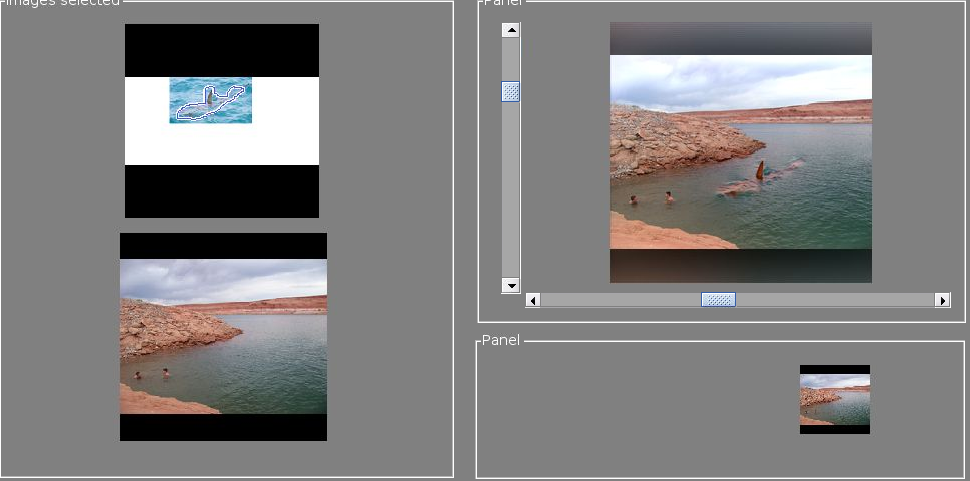
\includegraphics[width= 120pt]{Annexe/RequinF.png}
     \caption{Fourier}
   \end{minipage}
\end{figure}
%%%%%%%%%%%%%%%%%%%%OURS%%%%%%
\begin{figure}[!htb]
   \begin{minipage}{0.33\textwidth}
     \centering
     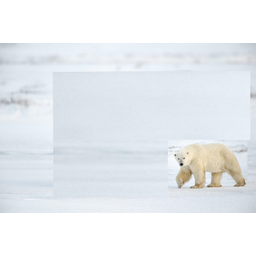
\includegraphics[width = 120pt]{Annexe/OursS.png}
     \caption{Image S}
      \end{minipage}\hfill
   \begin{minipage}{0.33\textwidth}
     \centering
     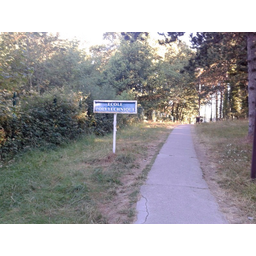
\includegraphics[width = 120pt]{Annexe/OursT.png}
     \caption{Image T}
      \end{minipage}\hfill
      \end{figure}

\begin{figure}[!htb]
   \begin{minipage}{0.33\textwidth}
     \centering
     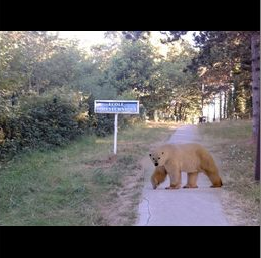
\includegraphics[width = 120pt]{Annexe/OursD.png}
     \caption{Méthode Douglas}
      \end{minipage}\hfill
   \begin{minipage}{0.33\textwidth}
     \centering
     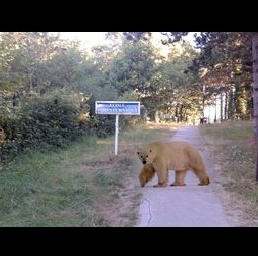
\includegraphics[width = 120pt]{Annexe/OursDF.png}
     \caption{Différences finies}
      \end{minipage}\hfill
   \begin{minipage}{0.33\textwidth}
     \centering
     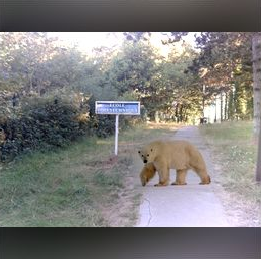
\includegraphics[width= 120pt]{Annexe/OursF.png}
     \caption{Fourier}
   \end{minipage}
\end{figure}


\end{document}
